\documentclass[12pt]{article}

%packages
%\usepackage{latexsym}
\usepackage{graphicx}
\usepackage{wrapfig}
\usepackage{color}
\usepackage{amsmath}
%\usepackage{dsfont}
\usepackage{placeins}
\usepackage{amssymb}
\usepackage{skull}
\usepackage{enumerate}
\usepackage{soul}
\usepackage{alphalph}
\usepackage{hyperref}
%\usepackage{fancyhdr}

%\fancyhf{} % clear all header and footers
%\renewcommand{\headrulewidth}{0pt} % remove the header rule
%\fancyfoot[LE, LO]{\thepage}


%\usepackage{pstricks,pst-node,pst-tree}

%\usepackage{algpseudocode}
%\usepackage{amsthm}
%\usepackage{hyperref}
%\usepackage{mathrsfs}
%\usepackage{amsfonts}
%\usepackage{bbding}
%\usepackage{listings}
%\usepackage{appendix}
\usepackage[margin=1in]{geometry}
%\geometry{papersize={8.5in,11in},total={6.5in,9in}}
%\usepackage{cancel}
%\usepackage{algorithmic, algorithm}

\newcommand{\qu}[1]{``#1''}
\newcommand{\spc}[1]{\\ \vspace{#1cm}}

\newcounter{probnum}
\setcounter{probnum}{1}
\newcounter{numpts}
\setcounter{numpts}{0}

%create definition to allow local margin changes
\def\changemargin#1#2{\list{}{\rightmargin#2\leftmargin#1}\item[]}
\let\endchangemargin=\endlist 

%allow equations to span multiple pages
\allowdisplaybreaks

%define colors and color typesetting conveniences
\definecolor{gray}{rgb}{0.5,0.5,0.5}
\definecolor{black}{rgb}{0,0,0}
\definecolor{white}{rgb}{1,1,1}
\definecolor{blue}{rgb}{0.5,0.5,1}
\newcommand{\inblue}[1]{\color{blue}#1 \color{black}}
\definecolor{green}{rgb}{0.133,0.545,0.133}
\newcommand{\ingreen}[1]{\color{green}#1 \color{black}}
\definecolor{yellow}{rgb}{1,0.549,0}
\newcommand{\inyellow}[1]{\color{yellow}#1 \color{black}}
\definecolor{red}{rgb}{1,0.133,0.133}
\newcommand{\inred}[1]{\color{red}#1 \color{black}}
\definecolor{purple}{rgb}{0.58,0,0.827}
\newcommand{\inpurple}[1]{\color{purple}#1 \color{black}}
\definecolor{gray}{rgb}{0.5,0.5,0.5}
\newcommand{\ingray}[1]{\color{gray}#1 \color{black}}
\definecolor{backgcode}{rgb}{0.97,0.97,0.8}
\definecolor{Brown}{cmyk}{0,0.81,1,0.60}
\definecolor{OliveGreen}{cmyk}{0.64,0,0.95,0.40}
\definecolor{CadetBlue}{cmyk}{0.62,0.57,0.23,0}

%define new math operators
\DeclareMathOperator*{\argmax}{arg\,max~}
\DeclareMathOperator*{\argmin}{arg\,min~}
\DeclareMathOperator*{\argsup}{arg\,sup~}
\DeclareMathOperator*{\arginf}{arg\,inf~}
\DeclareMathOperator*{\convolution}{\text{\Huge{$\ast$}}}
\newcommand{\infconv}[2]{\convolution^\infty_{#1 = 1} #2}
%true functions

%%%% GENERAL SHORTCUTS

\makeatletter
\newalphalph{\alphmult}[mult]{\@alph}{26}
\renewcommand{\labelenumi}{(\alphmult{\value{enumi}})}
\renewcommand{\theenumi}{\AlphAlph{\value{enumi}}}
\makeatother
%shortcuts for pure typesetting conveniences
\newcommand{\bv}[1]{\boldsymbol{#1}}

%shortcuts for compound constants
\newcommand{\BetaDistrConst}{\dfrac{\Gamma(\alpha + \beta)}{\Gamma(\alpha)\Gamma(\beta)}}
\newcommand{\NormDistrConst}{\dfrac{1}{\sqrt{2\pi\sigma^2}}}

%shortcuts for conventional symbols
\newcommand{\tsq}{\tau^2}
\newcommand{\tsqh}{\hat{\tau}^2}
\newcommand{\sigsq}{\sigma^2}
\newcommand{\sigsqsq}{\parens{\sigma^2}^2}
\newcommand{\sigsqovern}{\dfrac{\sigsq}{n}}
\newcommand{\tausq}{\tau^2}
\newcommand{\tausqalpha}{\tau^2_\alpha}
\newcommand{\tausqbeta}{\tau^2_\beta}
\newcommand{\tausqsigma}{\tau^2_\sigma}
\newcommand{\betasq}{\beta^2}
\newcommand{\sigsqvec}{\bv{\sigma}^2}
\newcommand{\sigsqhat}{\hat{\sigma}^2}
\newcommand{\sigsqhatmlebayes}{\sigsqhat_{\text{Bayes, MLE}}}
\newcommand{\sigsqhatmle}[1]{\sigsqhat_{#1, \text{MLE}}}
\newcommand{\bSigma}{\bv{\Sigma}}
\newcommand{\bSigmainv}{\bSigma^{-1}}
\newcommand{\thetavec}{\bv{\theta}}
\newcommand{\thetahat}{\hat{\theta}}
\newcommand{\thetahatmle}{\hat{\theta}_{\mathrm{MLE}}}
\newcommand{\thetavechatmle}{\hat{\thetavec}_{\mathrm{MLE}}}
\newcommand{\muhat}{\hat{\mu}}
\newcommand{\musq}{\mu^2}
\newcommand{\muvec}{\bv{\mu}}
\newcommand{\muhatmle}{\muhat_{\text{MLE}}}
\newcommand{\lambdahat}{\hat{\lambda}}
\newcommand{\lambdahatmle}{\lambdahat_{\text{MLE}}}
\newcommand{\thetahatmap}{\hat{\theta}_{\mathrm{MAP}}}
\newcommand{\thetahatmae}{\hat{\theta}_{\mathrm{MAE}}}
\newcommand{\thetahatmmse}{\hat{\theta}_{\mathrm{MMSE}}}
\newcommand{\etavec}{\bv{\eta}}
\newcommand{\alphavec}{\bv{\alpha}}
\newcommand{\minimaxdec}{\delta^*_{\mathrm{mm}}}
\newcommand{\ybar}{\bar{y}}
\newcommand{\xbar}{\bar{x}}
\newcommand{\Xbar}{\bar{X}}
\newcommand{\iid}{~{\buildrel iid \over \sim}~}
\newcommand{\inddist}{~{\buildrel ind \over \sim}~}
\newcommand{\approxdist}{~{\buildrel approx \over \sim}~}
\newcommand{\equalsindist}{~{\buildrel d \over =}~}
\newcommand{\loglik}[1]{\ell\parens{#1}}
\newcommand{\thetahatkminone}{\thetahat^{(k-1)}}
\newcommand{\thetahatkplusone}{\thetahat^{(k+1)}}
\newcommand{\thetahatk}{\thetahat^{(k)}}
\newcommand{\half}{\frac{1}{2}}
\newcommand{\third}{\frac{1}{3}}
\newcommand{\twothirds}{\frac{2}{3}}
\newcommand{\fourth}{\frac{1}{4}}
\newcommand{\fifth}{\frac{1}{5}}
\newcommand{\sixth}{\frac{1}{6}}

%shortcuts for vector and matrix notation
\newcommand{\A}{\bv{A}}
\newcommand{\At}{\A^T}
\newcommand{\Ainv}{\inverse{\A}}
\newcommand{\B}{\bv{B}}
\newcommand{\K}{\bv{K}}
\newcommand{\Kt}{\K^T}
\newcommand{\Kinv}{\inverse{K}}
\newcommand{\Kinvt}{(\Kinv)^T}
\newcommand{\M}{\bv{M}}
\newcommand{\Bt}{\B^T}
\newcommand{\Q}{\bv{Q}}
\newcommand{\Qt}{\Q^T}
\newcommand{\R}{\bv{R}}
\newcommand{\Rt}{\R^T}
\newcommand{\Z}{\bv{Z}}
\newcommand{\X}{\bv{X}}
\newcommand{\Xsub}{\X_{\text{(sub)}}}
\newcommand{\Xsubadj}{\X_{\text{(sub,adj)}}}
\newcommand{\I}{\bv{I}}
\newcommand{\Y}{\bv{Y}}
\newcommand{\sigsqI}{\sigsq\I}
\renewcommand{\P}{\bv{P}}
\newcommand{\Psub}{\P_{\text{(sub)}}}
\newcommand{\Pt}{\P^T}
\newcommand{\Pii}{P_{ii}}
\newcommand{\Pij}{P_{ij}}
\newcommand{\IminP}{(\I-\P)}
\newcommand{\Xt}{\bv{X}^T}
\newcommand{\XtX}{\Xt\X}
\newcommand{\XtXinv}{\parens{\Xt\X}^{-1}}
\newcommand{\XtXinvXt}{\XtXinv\Xt}
\newcommand{\XXtXinvXt}{\X\XtXinvXt}
\newcommand{\x}{\bv{x}}
\newcommand{\onevec}{\bv{1}}
\newcommand{\oneton}{1, \ldots, n}
\newcommand{\yoneton}{y_1, \ldots, y_n}
\newcommand{\yonetonorder}{y_{(1)}, \ldots, y_{(n)}}
\newcommand{\Yoneton}{Y_1, \ldots, Y_n}
\newcommand{\iinoneton}{i \in \braces{\oneton}}
\newcommand{\onetom}{1, \ldots, m}
\newcommand{\jinonetom}{j \in \braces{\onetom}}
\newcommand{\xoneton}{x_1, \ldots, x_n}
\newcommand{\Xoneton}{X_1, \ldots, X_n}
\newcommand{\xt}{\x^T}
\newcommand{\y}{\bv{y}}
\newcommand{\yt}{\y^T}
\renewcommand{\c}{\bv{c}}
\newcommand{\ct}{\c^T}
\newcommand{\tstar}{\bv{t}^*}
\renewcommand{\u}{\bv{u}}
\renewcommand{\v}{\bv{v}}
\renewcommand{\a}{\bv{a}}
\newcommand{\s}{\bv{s}}
\newcommand{\yadj}{\y_{\text{(adj)}}}
\newcommand{\xjadj}{\x_{j\text{(adj)}}}
\newcommand{\xjadjM}{\x_{j \perp M}}
\newcommand{\yhat}{\hat{\y}}
\newcommand{\yhatsub}{\yhat_{\text{(sub)}}}
\newcommand{\yhatstar}{\yhat^*}
\newcommand{\yhatstarnew}{\yhatstar_{\text{new}}}
\newcommand{\z}{\bv{z}}
\newcommand{\zt}{\z^T}
\newcommand{\bb}{\bv{b}}
\newcommand{\bbt}{\bb^T}
\newcommand{\bbeta}{\bv{\beta}}
\newcommand{\beps}{\bv{\epsilon}}
\newcommand{\bepst}{\beps^T}
\newcommand{\e}{\bv{e}}
\newcommand{\Mofy}{\M(\y)}
\newcommand{\KofAlpha}{K(\alpha)}
\newcommand{\ellset}{\mathcal{L}}
\newcommand{\oneminalph}{1-\alpha}
\newcommand{\SSE}{\text{SSE}}
\newcommand{\SSEsub}{\text{SSE}_{\text{(sub)}}}
\newcommand{\MSE}{\text{MSE}}
\newcommand{\RMSE}{\text{RMSE}}
\newcommand{\SSR}{\text{SSR}}
\newcommand{\SST}{\text{SST}}
\newcommand{\JSest}{\delta_{\text{JS}}(\x)}
\newcommand{\Bayesest}{\delta_{\text{Bayes}}(\x)}
\newcommand{\EmpBayesest}{\delta_{\text{EmpBayes}}(\x)}
\newcommand{\BLUPest}{\delta_{\text{BLUP}}}
\newcommand{\MLEest}[1]{\hat{#1}_{\text{MLE}}}

%shortcuts for Linear Algebra stuff (i.e. vectors and matrices)
\newcommand{\twovec}[2]{\bracks{\begin{array}{c} #1 \\ #2 \end{array}}}
\newcommand{\threevec}[3]{\bracks{\begin{array}{c} #1 \\ #2 \\ #3 \end{array}}}
\newcommand{\fivevec}[5]{\bracks{\begin{array}{c} #1 \\ #2 \\ #3 \\ #4 \\ #5 \end{array}}}
\newcommand{\twobytwomat}[4]{\bracks{\begin{array}{cc} #1 & #2 \\ #3 & #4 \end{array}}}
\newcommand{\threebytwomat}[6]{\bracks{\begin{array}{cc} #1 & #2 \\ #3 & #4 \\ #5 & #6 \end{array}}}

%shortcuts for conventional compound symbols
\newcommand{\thetainthetas}{\theta \in \Theta}
\newcommand{\reals}{\mathbb{R}}
\newcommand{\complexes}{\mathbb{C}}
\newcommand{\rationals}{\mathbb{Q}}
\newcommand{\integers}{\mathbb{Z}}
\newcommand{\naturals}{\mathbb{N}}
\newcommand{\forallninN}{~~\forall n \in \naturals}
\newcommand{\forallxinN}[1]{~~\forall #1 \in \reals}
\newcommand{\matrixdims}[2]{\in \reals^{\,#1 \times #2}}
\newcommand{\inRn}[1]{\in \reals^{\,#1}}
\newcommand{\mathimplies}{\quad\Rightarrow\quad}
\newcommand{\mathlogicequiv}{\quad\Leftrightarrow\quad}
\newcommand{\eqncomment}[1]{\quad \text{(#1)}}
\newcommand{\limitn}{\lim_{n \rightarrow \infty}}
\newcommand{\limitN}{\lim_{N \rightarrow \infty}}
\newcommand{\limitd}{\lim_{d \rightarrow \infty}}
\newcommand{\limitt}{\lim_{t \rightarrow \infty}}
\newcommand{\limitsupn}{\limsup_{n \rightarrow \infty}~}
\newcommand{\limitinfn}{\liminf_{n \rightarrow \infty}~}
\newcommand{\limitk}{\lim_{k \rightarrow \infty}}
\newcommand{\limsupn}{\limsup_{n \rightarrow \infty}}
\newcommand{\limsupk}{\limsup_{k \rightarrow \infty}}
\newcommand{\floor}[1]{\left\lfloor #1 \right\rfloor}
\newcommand{\ceil}[1]{\left\lceil #1 \right\rceil}

%shortcuts for environments
\newcommand{\beqn}{\vspace{-0.25cm}\begin{eqnarray*}}
\newcommand{\eeqn}{\end{eqnarray*}}
\newcommand{\bneqn}{\vspace{-0.25cm}\begin{eqnarray}}
\newcommand{\eneqn}{\end{eqnarray}}
\newcommand{\benum}{\begin{enumerate}}
\newcommand{\eenum}{\end{enumerate}}

%shortcuts for mini environments
\newcommand{\parens}[1]{\left(#1\right)}
\newcommand{\squared}[1]{\parens{#1}^2}
\newcommand{\tothepow}[2]{\parens{#1}^{#2}}
\newcommand{\prob}[1]{\mathbb{P}\parens{#1}}
\newcommand{\littleo}[1]{o\parens{#1}}
\newcommand{\bigo}[1]{O\parens{#1}}
\newcommand{\Lp}[1]{\mathbb{L}^{#1}}
\renewcommand{\arcsin}[1]{\text{arcsin}\parens{#1}}
\newcommand{\prodonen}[2]{\bracks{\prod_{#1=1}^n #2}}
\newcommand{\mysum}[4]{\sum_{#1=#2}^{#3} #4}
\newcommand{\sumonen}[2]{\sum_{#1=1}^n #2}
\newcommand{\infsum}[2]{\sum_{#1=1}^\infty #2}
\newcommand{\infprod}[2]{\prod_{#1=1}^\infty #2}
\newcommand{\infunion}[2]{\bigcup_{#1=1}^\infty #2}
\newcommand{\infinter}[2]{\bigcap_{#1=1}^\infty #2}
\newcommand{\infintegral}[2]{\int^\infty_{-\infty} #2 ~\text{d}#1}
\newcommand{\supthetas}[1]{\sup_{\thetainthetas}\braces{#1}}
\newcommand{\bracks}[1]{\left[#1\right]}
\newcommand{\braces}[1]{\left\{#1\right\}}
\newcommand{\set}[1]{\left\{#1\right\}}
\newcommand{\abss}[1]{\left|#1\right|}
\newcommand{\norm}[1]{\left|\left|#1\right|\right|}
\newcommand{\normsq}[1]{\norm{#1}^2}
\newcommand{\inverse}[1]{\parens{#1}^{-1}}
\newcommand{\rowof}[2]{\parens{#1}_{#2\cdot}}

%shortcuts for functionals
\newcommand{\realcomp}[1]{\text{Re}\bracks{#1}}
\newcommand{\imagcomp}[1]{\text{Im}\bracks{#1}}
\newcommand{\range}[1]{\text{range}\bracks{#1}}
\newcommand{\colsp}[1]{\text{colsp}\bracks{#1}}
\newcommand{\rowsp}[1]{\text{rowsp}\bracks{#1}}
\newcommand{\tr}[1]{\text{tr}\bracks{#1}}
\newcommand{\rank}[1]{\text{rank}\bracks{#1}}
\newcommand{\proj}[2]{\text{Proj}_{#1}\bracks{#2}}
\newcommand{\projcolspX}[1]{\text{Proj}_{\colsp{\X}}\bracks{#1}}
\newcommand{\median}[1]{\text{median}\bracks{#1}}
\newcommand{\mean}[1]{\text{mean}\bracks{#1}}
\newcommand{\dime}[1]{\text{dim}\bracks{#1}}
\renewcommand{\det}[1]{\text{det}\bracks{#1}}
\newcommand{\expe}[1]{\mathbb{E}\bracks{#1}}
\newcommand{\expeabs}[1]{\expe{\abss{#1}}}
\newcommand{\expesub}[2]{\mathbb{E}_{#1}\bracks{#2}}
\newcommand{\cexpesub}[3]{\mathbb{E}_{#1}\bracks{#2~|~#3}}
\newcommand{\indic}[1]{\mathds{1}_{#1}}
\newcommand{\var}[1]{\mathbb{V}\text{ar}\bracks{#1}}
\newcommand{\sd}[1]{\mathbb{S}\text{D}\bracks{#1}}
\newcommand{\cov}[2]{\text{Cov}\bracks{#1, #2}}
\newcommand{\corr}[2]{\text{Corr}\bracks{#1, #2}}
\newcommand{\se}[1]{\text{SE}\bracks{#1}}
\newcommand{\seest}[1]{\hat{\text{SE}}\bracks{#1}}
\newcommand{\bias}[1]{\text{Bias}\bracks{#1}}
\newcommand{\partialop}[2]{\dfrac{\partial}{\partial #1}\bracks{#2}}
\newcommand{\secpartialop}[2]{\dfrac{\partial^2}{\partial #1^2}\bracks{#2}}
\newcommand{\mixpartialop}[3]{\dfrac{\partial^2}{\partial #1 \partial #2}\bracks{#3}}

%shortcuts for functions
\renewcommand{\exp}[1]{\mathrm{exp}\parens{#1}}
\renewcommand{\cos}[1]{\text{cos}\parens{#1}}
\renewcommand{\sin}[1]{\text{sin}\parens{#1}}
\newcommand{\sign}[1]{\text{sign}\parens{#1}}
\newcommand{\are}[1]{\mathrm{ARE}\parens{#1}}
\newcommand{\natlog}[1]{\ln\parens{#1}}
\newcommand{\oneover}[1]{\frac{1}{#1}}
\newcommand{\overtwo}[1]{\frac{#1}{2}}
\newcommand{\overn}[1]{\frac{#1}{n}}
\newcommand{\oneoversqrt}[1]{\oneover{\sqrt{#1}}}
\newcommand{\sqd}[1]{\parens{#1}^2}
\newcommand{\loss}[1]{\ell\parens{\theta, #1}}
\newcommand{\losstwo}[2]{\ell\parens{#1, #2}}
\newcommand{\cf}{\phi(t)}

%English language specific shortcuts
\newcommand{\ie}{\textit{i.e.} }
\newcommand{\AKA}{\textit{AKA} }
\renewcommand{\iff}{\textit{iff}}
\newcommand{\eg}{\textit{e.g.} }
\renewcommand{\st}{\textit{s.t.} }
\newcommand{\wrt}{\textit{w.r.t.} }
\newcommand{\mathst}{~~\text{\st}~~}
\newcommand{\mathand}{~~\text{and}~~}
\newcommand{\ala}{\textit{a la} }
\newcommand{\ppp}{posterior predictive p-value}
\newcommand{\dd}{dataset-to-dataset}

%shortcuts for distribution titles
\newcommand{\logistic}[2]{\mathrm{Logistic}\parens{#1,\,#2}}
\newcommand{\bernoulli}[1]{\mathrm{Bernoulli}\parens{#1}}
\newcommand{\betanot}[2]{\mathrm{Beta}\parens{#1,\,#2}}
\newcommand{\stdbetanot}{\betanot{\alpha}{\beta}}
\newcommand{\multnormnot}[3]{\mathcal{N}_{#1}\parens{#2,\,#3}}
\newcommand{\normnot}[2]{\mathcal{N}\parens{#1,\,#2}}
\newcommand{\classicnormnot}{\normnot{\mu}{\sigsq}}
\newcommand{\stdnormnot}{\normnot{0}{1}}
\newcommand{\uniform}[2]{\mathrm{U}\parens{#1,\,#2}}
\newcommand{\stduniform}{\uniform{0}{1}}
\newcommand{\exponential}[1]{\mathrm{Exp}\parens{#1}}
\newcommand{\gammadist}[2]{\mathrm{Gamma}\parens{#1, #2}}
\newcommand{\poisson}[1]{\mathrm{Poisson}\parens{#1}}
\newcommand{\binomial}[2]{\mathrm{Binomial}\parens{#1,\,#2}}
\newcommand{\rayleigh}[1]{\mathrm{Rayleigh}\parens{#1}}
\newcommand{\multinomial}[2]{\mathrm{Multinomial}\parens{#1,\,#2}}
\newcommand{\gammanot}[2]{\mathrm{Gamma}\parens{#1,\,#2}}
\newcommand{\cauchynot}[2]{\text{Cauchy}\parens{#1,\,#2}}
\newcommand{\invchisqnot}[1]{\text{Inv}\chisq{#1}}
\newcommand{\invscaledchisqnot}[2]{\text{ScaledInv}\ncchisq{#1}{#2}}
\newcommand{\invgammanot}[2]{\text{InvGamma}\parens{#1,\,#2}}
\newcommand{\chisq}[1]{\chi^2_{#1}}
\newcommand{\ncchisq}[2]{\chi^2_{#1}\parens{#2}}
\newcommand{\ncF}[3]{F_{#1,#2}\parens{#3}}

%shortcuts for PDF's of common distributions
\newcommand{\logisticpdf}[3]{\oneover{#3}\dfrac{\exp{-\dfrac{#1 - #2}{#3}}}{\parens{1+\exp{-\dfrac{#1 - #2}{#3}}}^2}}
\newcommand{\betapdf}[3]{\dfrac{\Gamma(#2 + #3)}{\Gamma(#2)\Gamma(#3)}#1^{#2-1} (1-#1)^{#3-1}}
\newcommand{\normpdf}[3]{\frac{1}{\sqrt{2\pi#3}}\exp{-\frac{1}{2#3}(#1 - #2)^2}}
\newcommand{\normpdfvarone}[2]{\dfrac{1}{\sqrt{2\pi}}e^{-\half(#1 - #2)^2}}
\newcommand{\chisqpdf}[2]{\dfrac{1}{2^{#2/2}\Gamma(#2/2)}\; {#1}^{#2/2-1} e^{-#1/2}}
\newcommand{\invchisqpdf}[2]{\dfrac{2^{-\overtwo{#1}}}{\Gamma(#2/2)}\,{#1}^{-\overtwo{#2}-1}  e^{-\oneover{2 #1}}}
\newcommand{\uniformdiscrete}[1]{\mathrm{Uniform}\parens{\braces{#1}}}
\newcommand{\exponentialpdf}[2]{#2\exp{-#2#1}}
\newcommand{\poissonpdf}[2]{\dfrac{e^{-#1} #1^{#2}}{#2!}}
\newcommand{\binomialpdf}[3]{\binom{#2}{#1}#3^{#1}(1-#3)^{#2-#1}}
\newcommand{\rayleighpdf}[2]{\dfrac{#1}{#2^2}\exp{-\dfrac{#1^2}{2 #2^2}}}
\newcommand{\gammapdf}[3]{\dfrac{#3^#2}{\Gamma\parens{#2}}#1^{#2-1}\exp{-#3 #1}}
\newcommand{\cauchypdf}[3]{\oneover{\pi} \dfrac{#3}{\parens{#1-#2}^2 + #3^2}}
\newcommand{\Gammaf}[1]{\Gamma\parens{#1}}

%shortcuts for miscellaneous typesetting conveniences
\newcommand{\notesref}[1]{\marginpar{\color{gray}\tt #1\color{black}}}

%%%% DOMAIN-SPECIFIC SHORTCUTS

%Real analysis related shortcuts
\newcommand{\zeroonecl}{\bracks{0,1}}
\newcommand{\forallepsgrzero}{\forall \epsilon > 0~~}
\newcommand{\lessthaneps}{< \epsilon}
\newcommand{\fraccomp}[1]{\text{frac}\bracks{#1}}

%Bayesian related shortcuts
\newcommand{\yrep}{y^{\text{rep}}}
\newcommand{\yrepisq}{(\yrep_i)^2}
\newcommand{\yrepvec}{\bv{y}^{\text{rep}}}


%Probability shortcuts
\newcommand{\SigField}{\mathcal{F}}
\newcommand{\ProbMap}{\mathcal{P}}
\newcommand{\probtrinity}{\parens{\Omega, \SigField, \ProbMap}}
\newcommand{\convp}{~{\buildrel p \over \rightarrow}~}
\newcommand{\convLp}[1]{~{\buildrel \Lp{#1} \over \rightarrow}~}
\newcommand{\nconvp}{~{\buildrel p \over \nrightarrow}~}
\newcommand{\convae}{~{\buildrel a.e. \over \longrightarrow}~}
\newcommand{\convau}{~{\buildrel a.u. \over \longrightarrow}~}
\newcommand{\nconvau}{~{\buildrel a.u. \over \nrightarrow}~}
\newcommand{\nconvae}{~{\buildrel a.e. \over \nrightarrow}~}
\newcommand{\convd}{~{\buildrel \mathcal{D} \over \rightarrow}~}
\newcommand{\nconvd}{~{\buildrel \mathcal{D} \over \nrightarrow}~}
\newcommand{\withprob}{~~\text{w.p.}~~}
\newcommand{\io}{~~\text{i.o.}}

\newcommand{\Acl}{\bar{A}}
\newcommand{\ENcl}{\bar{E}_N}
\newcommand{\diam}[1]{\text{diam}\parens{#1}}

\newcommand{\taua}{\tau_a}

\newcommand{\myint}[4]{\int_{#2}^{#3} #4 \,\text{d}#1}
\newcommand{\laplacet}[1]{\mathscr{L}\bracks{#1}}
\newcommand{\laplaceinvt}[1]{\mathscr{L}^{-1}\bracks{#1}}
\renewcommand{\min}[1]{\text{min}\braces{#1}}

\newcommand{\Vbar}[1]{\bar{V}\parens{#1}}
\newcommand{\expnegrtau}{\exp{-r\tau}}
\newcommand{\cprob}[2]{\prob{#1~|~#2}}

%%% problem typesetting
\newcommand{\problem}{\vspace{0.2cm} \noindent {\large{\textsf{Problem \arabic{probnum}~}}} \addtocounter{probnum}{1}}
%\newcommand{\easyproblem}{\ingreen{\noindent \textsf{Problem \arabic{probnum}~}} \addtocounter{probnum}{1}}
%\newcommand{\intermediateproblem}{\noindent \inyellow{\textsf{Problem \arabic{probnum}~}} \addtocounter{probnum}{1}}
%\newcommand{\hardproblem}{\inred{\noindent \textsf{Problem \arabic{probnum}~}} \addtocounter{probnum}{1}}
%\newcommand{\extracreditproblem}{\noindent \inpurple{\textsf{Problem \arabic{probnum}~}} \addtocounter{probnum}{1}}

\newcommand{\easysubproblem}{\ingreen{\item}}
\newcommand{\intermediatesubproblem}{\inyellow{\item}}
\newcommand{\hardsubproblem}{\inred{\item}}
\newcommand{\extracreditsubproblem}{\inpurple{\item}}
%\newcommand{\subquestionwithpoints}[1]{\addtocounter{numpts}{#1} \item \ingray{[#1 pt]}~~} %  / \arabic{numpts} pts
\newcommand{\subquestionwithpoints}[1]{\addtocounter{numpts}{#1} \item \ingray{[#1 pt / \arabic{numpts} pts]}~~}  

\title{Math 341 / 650 Spring 2019 \\ Final Examination}
\author{Professor Adam Kapelner}

\date{Thursday, May 16, 2019}

\begin{document}
\maketitle

\noindent Full Name \line(1,0){410}

\thispagestyle{empty}

\section*{Code of Academic Integrity}

\footnotesize
Since the college is an academic community, its fundamental purpose is the pursuit of knowledge. Essential to the success of this educational mission is a commitment to the principles of academic integrity. Every member of the college community is responsible for upholding the highest standards of honesty at all times. Students, as members of the community, are also responsible for adhering to the principles and spirit of the following Code of Academic Integrity.

Activities that have the effect or intention of interfering with education, pursuit of knowledge, or fair evaluation of a student's performance are prohibited. Examples of such activities include but are not limited to the following definitions:

\paragraph{Cheating} Using or attempting to use unauthorized assistance, material, or study aids in examinations or other academic work or preventing, or attempting to prevent, another from using authorized assistance, material, or study aids. Example: using an unauthorized cheat sheet in a quiz or exam, altering a graded exam and resubmitting it for a better grade, etc.
\\

\noindent I acknowledge and agree to uphold this Code of Academic Integrity. \\

\begin{center}
\line(1,0){250} ~~~ \line(1,0){100}\\
~~~~~~~~~~~~~~~~~~~~~signature~~~~~~~~~~~~~~~~~~~~~~~~~~~~~~~~~~~~~~~~~~~~~ date
\end{center}

\normalsize

\section*{Instructions}

This exam is 120 minutes and closed-book. You are allowed \textbf{three} pages (front and back) of a \qu{cheat sheet.} You may use a graphing calculator of your choice. Please read the questions carefully. If the question reads \qu{compute,} this means the solution will be a number otherwise you can leave the answer in \textit{any} widely accepted mathematical notation which could be resolved to an exact or approximate number with the use of a computer. I advise you to skip problems marked \qu{[Extra Credit]} until you have finished the other questions on the exam, then loop back and plug in all the holes. I also advise you to use pencil. The exam is 100 points total plus extra credit. Partial credit will be granted for incomplete answers on most of the questions. \fbox{Box} in your final answers. Good luck!

\pagebreak


\begin{table}[htp]
\centering
\small
\begin{tabular}{l | llll}
Distribution                  & Quantile  & PMF / PDF  &CDF       & Sampling  \\ 
of r.v. &  Function & function         & function &  Function \\ \hline
beta & \texttt{qbeta}($p$, $\alpha$, $\beta$)             
& \texttt{d-}($x$, $\alpha$, $\beta$)
& \texttt{p-}($x$, $\alpha$, $\beta$) 
& \texttt{r-}($\alpha$, $\beta$) \\
betabinomial & \texttt{qbetabinom}($p$, $n$, $\alpha$, $\beta$)              
& \texttt{d-}($x$, $n$, $\alpha$, $\beta$)
& \texttt{p-}($x$, $n$, $\alpha$, $\beta$) 
& \texttt{r-}($n$, $\alpha$, $\beta$) \\

%betanegativebinomial & \texttt{qbeta\_nbinom}($p$, $r$, $\alpha$, $\beta$) 
%& \texttt{d-}($x$, $r$, $\alpha$, $\beta$)
%& \texttt{p-}($x$, $r$, $\alpha$, $\beta$) 
%& \texttt{r-}($r$, $\alpha$, $\beta$) \\

binomial & \texttt{qbinom}($p$, $n$, $\theta$) 
& \texttt{d-}($x$, $n$, $\theta$)
& \texttt{p-}($x$, $n$, $\theta$) 
& \texttt{r-}($n$, $\theta$) \\

exponential & \texttt{qexp}($p$, $\theta$) 
& \texttt{d-}($x$, $\theta$) 
& \texttt{p-}($x$, $\theta$) 
& \texttt{r-}($\theta$) \\

gamma & \texttt{qgamma}($p$, $\alpha$, $\beta$) 
& \texttt{d-}($x$, $\alpha$, $\beta$)
& \texttt{p-}($x$, $\alpha$, $\beta$) 
& \texttt{r-}($\alpha$, $\beta$) \\

%geometric & \texttt{qgeom}($p$, $\theta$) 
%& \texttt{d-}($x$, $\theta$)
%& \texttt{p-}($x$, $\theta$) 
%& \texttt{r-}($\theta$) \\

inversegamma & \texttt{qinvgamma}($p$, $\alpha$, $\beta$) 
& \texttt{d-}($x$, $\alpha$, $\beta$)
& \texttt{p-}($x$, $\alpha$, $\beta$) 
& \texttt{r-}($\alpha$, $\beta$) \\

negative-binomial & \texttt{qnbinom}($p$, $r$, $\theta$) 
& \texttt{d-}($x$, $r$, $\theta$) 
& \texttt{p-}($x$, $r$, $\theta$) 
& \texttt{r-}($r$, $\theta$) \\

normal (univariate) & \texttt{qnorm}($p$, $\theta$, $\sigma$) 
& \texttt{d-}($x$, $\theta$, $\sigma$)
& \texttt{p-}($x$, $\theta$, $\sigma$) 
& \texttt{r-}($\theta$, $\sigma$) \\

%normal (multivariate) & 
%& \multicolumn{2}{l}{\texttt{dmvnorm}($\x$, $\muvec$, $\bSigma$)} 
%& \texttt{r-}($\muvec$, $\bSigma$) \\

poisson & \texttt{qpois}($p$, $\theta$) 
& \texttt{d-}($x$, $\theta$)
& \texttt{p-}($x$, $\theta$) 
& \texttt{r-}($\theta$) \\

T (standard) & \texttt{qt}($p$, $\nu$) 
& \texttt{d-}($x$, $\nu$) 
& \texttt{p-}($x$, $\nu$)
& \texttt{r-}($\nu$) \\

T (nonstandard) & \texttt{qt.scaled}($p$, $\nu$, $\mu$, $\sigma$) 
& \texttt{d-}($x$, $\nu$, $\mu$, $\sigma$)
& \texttt{p-}($x$, $\nu$, $\mu$, $\sigma$) 
& \texttt{r-}($\nu$, $\mu$, $\sigma$) \\

uniform & \texttt{qunif}($p$, $a$, $b$) 
& \texttt{d-}($x$, $a$, $b$)
& \texttt{p-}($x$, $a$, $b$) 
& \texttt{r-}($a$, $b$) \\


\end{tabular}
\caption{Functions from $\texttt{R}$ (in alphabetical order) that can be used on this assignment and exams. The hyphen in colums 3, 4 and 5 is shorthand notation for the full text of the r.v. which can be found in column 2.
}
\label{tab:eqs}
\end{table}

\problem Consider a call center that experiences calls from a large population of which there is very small probability each customer will call in each day. Let $\Xoneton$ denote the number of calls in a period of $n$ days. However, there are two types of customers: A and B (since there are two main products the company offers). And thus each day is either calls from company A or B:

\beqn
\Xoneton~|~\lambda_1, \lambda_2, \rho ~\iid~ \begin{cases} \frac{e^{-\lambda_1}\lambda_1^x}{x!} ~~w.p.~~\rho \\
\frac{e^{-\lambda_2}\lambda_2^x}{x!} ~~w.p.~~(1-\rho) 
\end{cases}
\eeqn

\benum
\subquestionwithpoints{6} Provide uninformative priors for the three parameters. \spc{3}

We now introduce the new parameters $I_1, \ldots, I_n$ where each is defined as:

\beqn
I_i := \begin{cases}
1 ~~\text{if the calls from day $i$ come from customer type A} \\
0 ~~\text{if the calls from day $i$ come from customer type B} \\
\end{cases}
\eeqn

This is an idea known as \qu{data augmentation}. The likelihood now  becomes:

\beqn
&& \cprob{X_1, \ldots, X_n}{\lambda_1, \lambda_2, \rho, I_1, \ldots, I_n} = \prod_{i=1}^n \tothepow{\frac{e^{-\lambda_1}\lambda_1^{x_i}}{x_i!}}{I_i} \tothepow{\frac{e^{-\lambda_2}\lambda_2^{x_i}}{x_i!}}{1 - I_i} \rho^{I_i} (1 - \rho)^{1 - I_i} 
\eeqn


\subquestionwithpoints{5} Denote $\sum I_i := \sum_{i=1}^n I_i$. By using the likelihood above and your priors from part (a), Show all your work to prove that the kernel of $\cprob{\lambda_1, \lambda_2, \rho, I_1, \ldots, I_n}{X_1, \ldots, X_n}$, the posterior  is

\vspace{-0.5cm}
\beqn
e^{-(\sum I_i) \lambda_1 } \lambda_1^{\sum I_i x_i} e^{-(n - \sum I_i) \lambda_2 } \lambda_2^{\sum (1 - I_i) x_i} \rho^{\sum I_i} (1 - \rho)^{n - \sum I_i}
\eeqn\spc{4}

\subquestionwithpoints{2} Is this a kernel from a known distribution? Yes / no. \spc{-0.5}


\subquestionwithpoints{4} Name two strategies that can be used to creates samples $\bracks{\lambda_1, \lambda_2, \rho, I_1, \ldots, I_n}$ from the posterior $\cprob{\lambda_1, \lambda_2, \rho, I_1, \ldots, I_n}{X_1, \ldots, X_n}$. \spc{1}

\subquestionwithpoints{4} Which strategy would be better and why? \spc{2}

\subquestionwithpoints{4} Find the conditional distribution $\cprob{\lambda_1}{X_1, \ldots, X_n, \lambda_2, \rho, I_1, \ldots, I_n}$. If the PMF / PDF are from a known, brand name random variable, name the distribution and provide its parameter(s). Show all work. \spc{2}

\subquestionwithpoints{4} Find the conditional distribution $\cprob{\lambda_2}{X_1, \ldots, X_n, \lambda_1, \rho, I_1, \ldots, I_n}$. If the PMF / PDF are from a known, brand name random variable, name the distribution and provide its parameter(s). Show all work.\spc{2}

\subquestionwithpoints{6} Find the conditional distribution $\cprob{\rho}{X_1, \ldots, X_n, \lambda_1, \lambda_2, I_1, \ldots, I_n}$. If the PMF / PDF is from a known, brand name random variable, name the distribution and provide its parameter(s). Show all work.\spc{4}


\subquestionwithpoints{5} [Extra Credit] Find the conditional distribution for $I_1$ given the data and the other parameters. If the PMF / PDF is from a known, brand name random variable, name the distribution and provide its parameter(s). Show all work.\spc{6}

Below is a bar plot of our data for $n = 300$ days:

\begin{figure}[h]
\centering
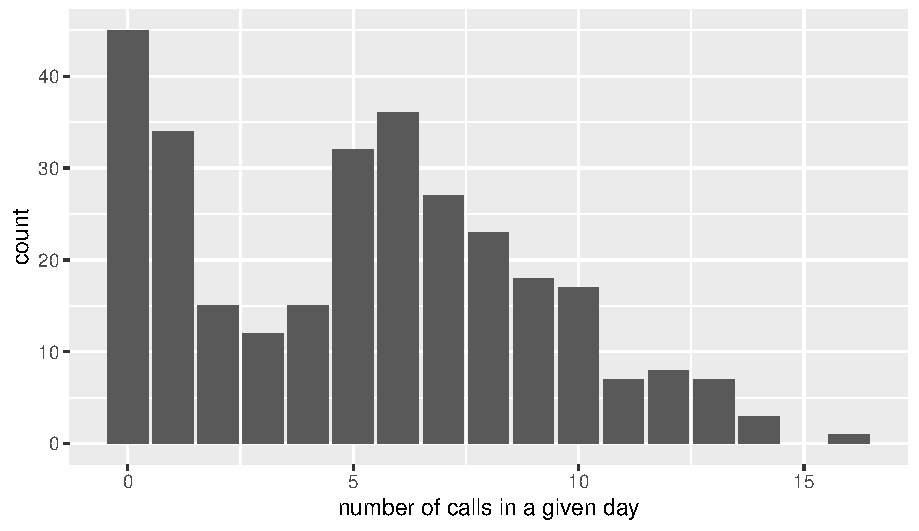
\includegraphics[width=4.9in]{data_barplot}
\end{figure}
\FloatBarrier

We now build a Gibbs Sampler for all parameters $\lambda_1, \lambda_2, \rho, I_1, \ldots, I_n$ based on your answers from (a)-(h) and initially sample $10,000$ times. Below is the first 50 samples from the chains for $\lambda_1, \lambda_2, \rho$:

\begin{figure}[h]
\centering
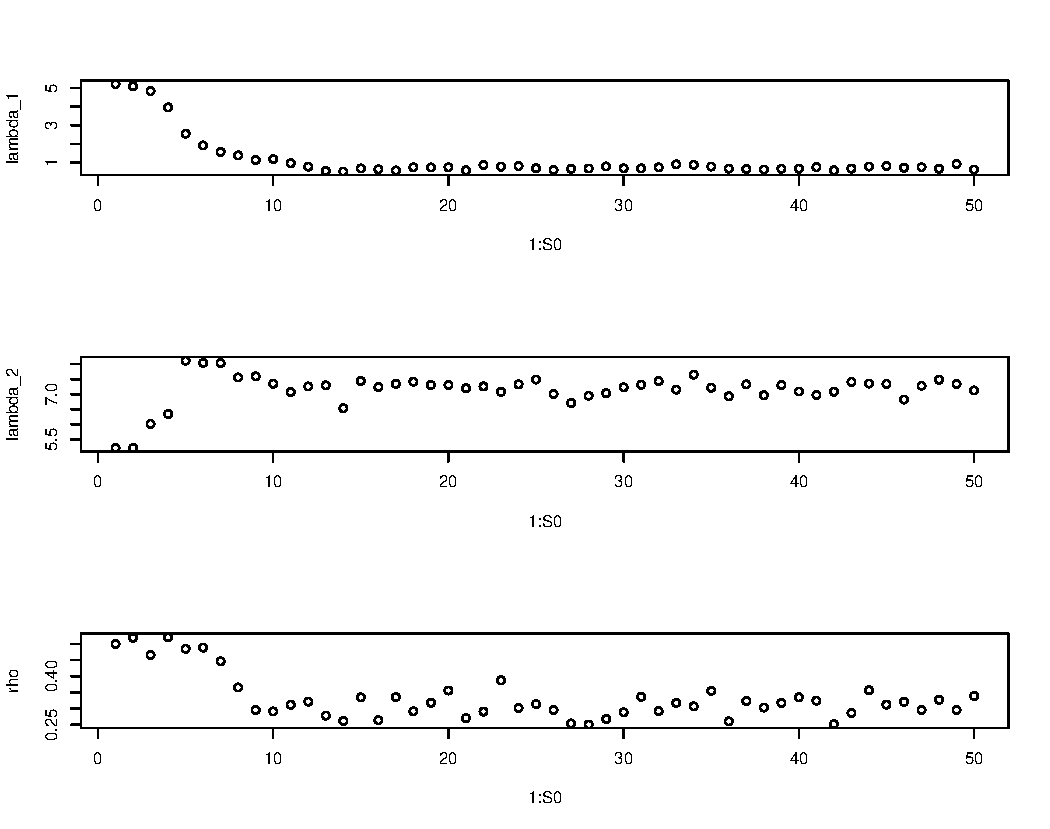
\includegraphics[width=7.5in]{burn_in}
\end{figure}
\FloatBarrier

\subquestionwithpoints{3} How many of the initial samples should be thrown away? \spc{7}

After removing the initial part of the chain according to your answer in the previous question, below is an autocorrelation plot of the chains for $\lambda_1, \lambda_2, \rho$ with maximum lag 10:

\begin{figure}[h]
\centering
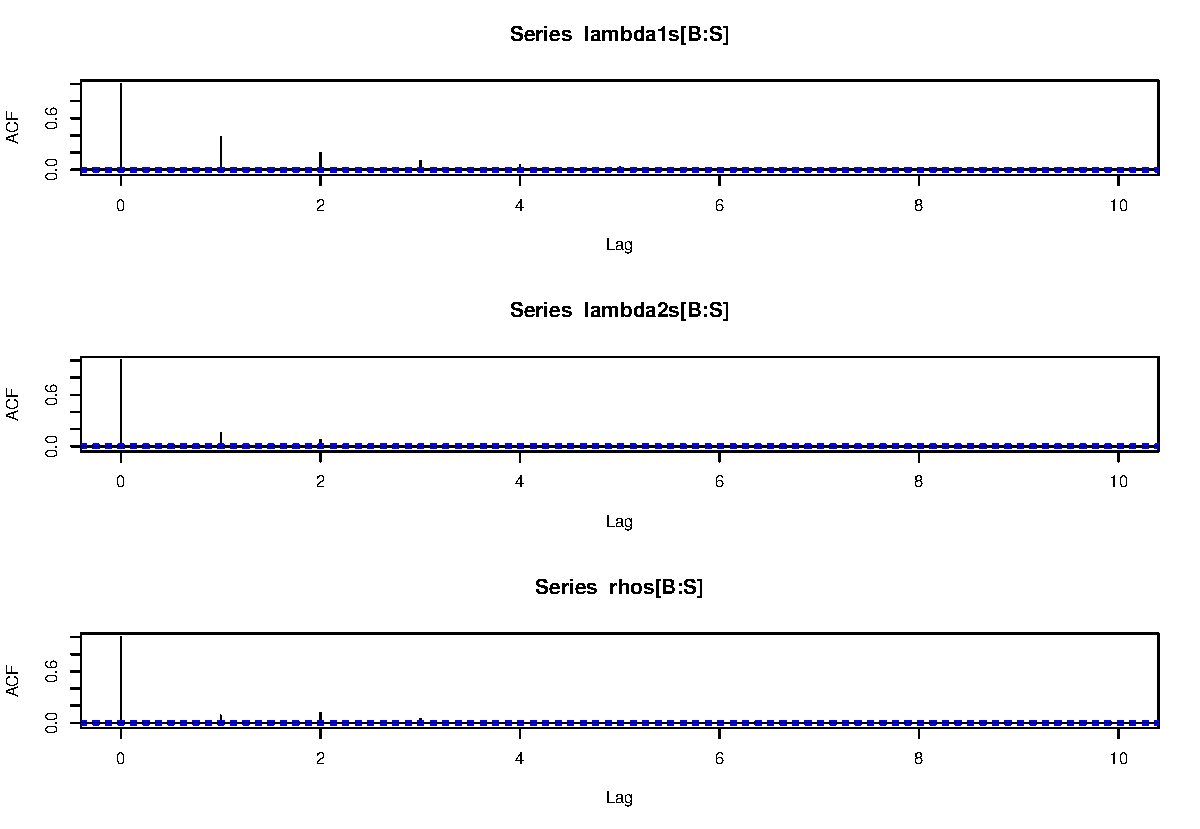
\includegraphics[width=7.5in]{acf}
\end{figure}
\FloatBarrier

\subquestionwithpoints{3} How many iterations do you think should be skipped between samples in the burned-in chains if you want $\iid$ samples from the posterior? \spc{1}

\subquestionwithpoints{4} How many $\iid$ samples from the posterior do you have now? \spc{2}

The next page shows four different histograms: one for each of the burned and thinned chains for $\lambda_1, \lambda_2, \rho$ and $I_{31}$.

\begin{figure}[h]
\centering
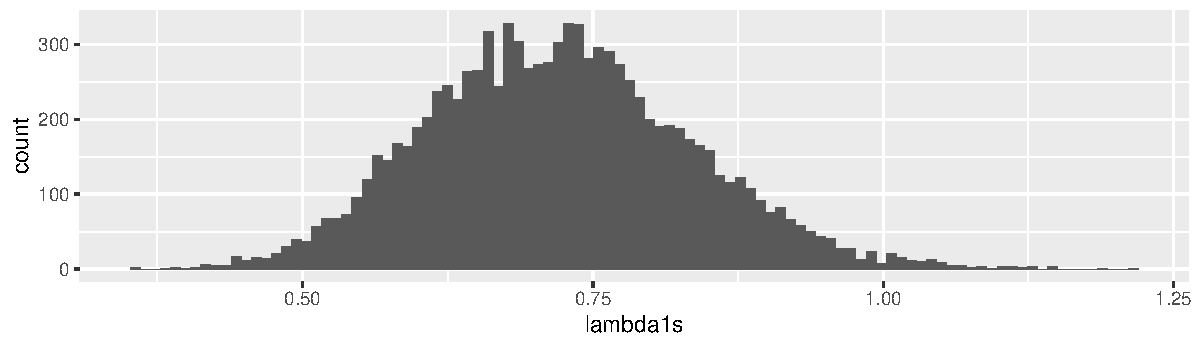
\includegraphics[width=7in]{lambda1s}
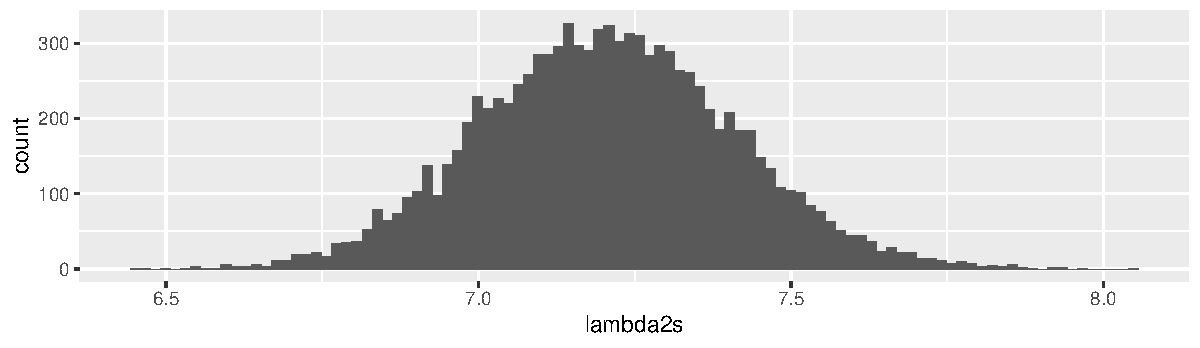
\includegraphics[width=7in]{lambda2s}
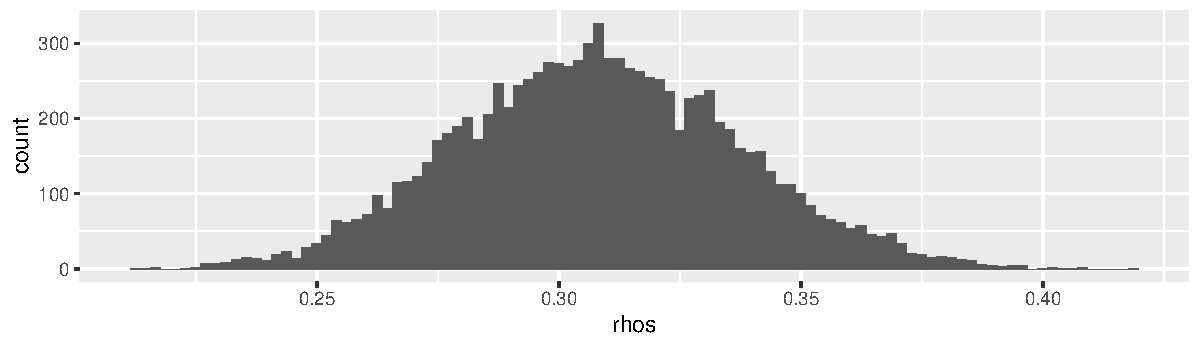
\includegraphics[width=7in]{rhos}
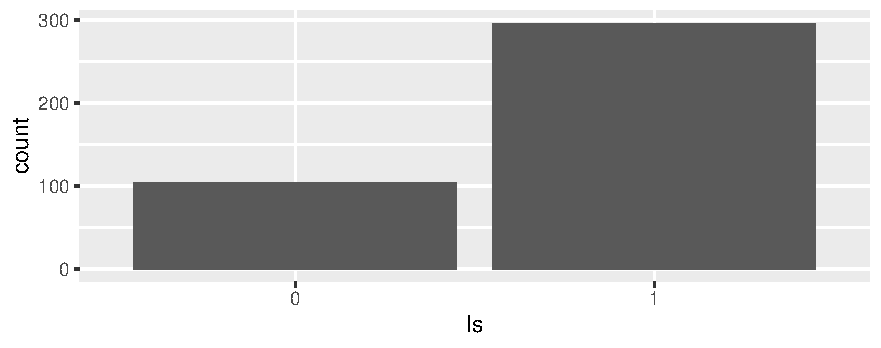
\includegraphics[width=5in]{I31}
\end{figure}
\FloatBarrier


\subquestionwithpoints{6} Provide an approximate $CR_{\lambda_1, 90\%}$. \spc{4}

\subquestionwithpoints{5} Provide an approximate Bayesian point estimate for $\lambda_2$. Indicate which point estimate you are providing by specifying the subscript to $\thetahat$. \spc{4}

\subquestionwithpoints{8} Test $\rho \neq 0.3$ using $\delta = 0.05$. List the hypotheses, pick an $\alpha$ level and provide an approximate Bayesian $p$-value and give a one sentence interpretation of the test result. \spc{7}

\subquestionwithpoints{4} In your estimation, what type of customer dominates day 31's phone calls? \spc{1}




\subquestionwithpoints{8} Explain how you would provide \emph{one} prediction for the next day's number of phone calls. Clearly write out all your steps. Make sure the company can run your code. The functions you use from Table~\ref{tab:eqs} must have explicit numeric values.  Below are 10 random samples from the burned and thinned chains for parameters $\lambda_1, \lambda_2, \rho$:

 
\begin{verbatim}
          [,1]  [,2]  [,3]  [,4]  [,5]  [,6]  [,7]  [,8]  [,9] [,10]
lambda1s 0.731 0.573 0.861 0.770 0.797 0.683 0.597 0.649 0.670 0.784
lambda2s 7.312 7.203 7.259 7.077 7.328 7.489 7.006 6.709 6.950 7.036
rhos     0.356 0.271 0.291 0.388 0.301 0.314 0.296 0.254 0.251 0.260
\end{verbatim}

Your answer must use some of the above numbers somehow.\spc{9}


\eenum

\problem This question is about building a model to understand the accuracy of this beverage-filling machine

\begin{figure}[htp]
\centering
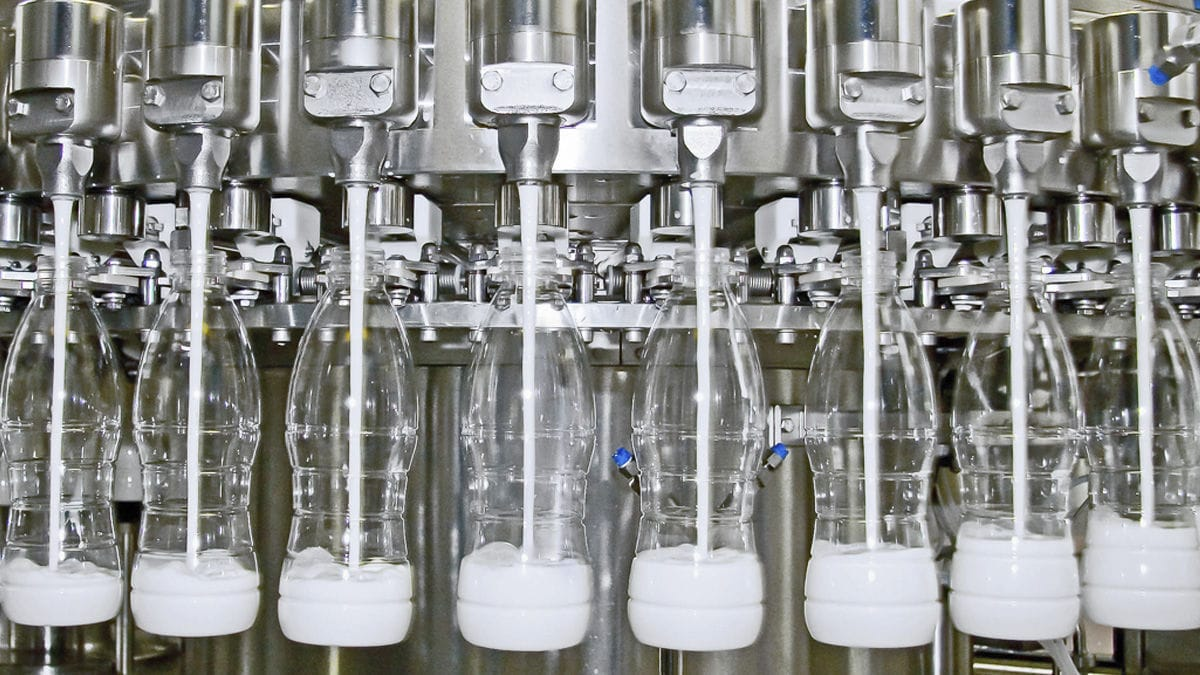
\includegraphics[width=2.4in]{milk_filling.jpg}
\end{figure}

\noindent which fills 12oz plastic bottles. We decide to do an experiment and select $n = 20$ bottles at random and measure the amount of liquid in each bottle. Here are the volumes (in oz):

\begin{verbatim}
       10.76 11.02 11.62 10.20 12.03 12.18 12.06 11.42 11.93 10.68
       11.81 11.27 11.68 11.31 11.29 12.37 12.00 10.74 12.04 10.69
\end{verbatim}

\noindent and sample statistics: $\xbar = 11.6$oz and $s = 0.53$oz. We will consider these measurements realizations from $\mathcal{F} : \Xoneton~|~\theta, \sigsq \iid \normnot{\theta}{\sigsq}$ where both $\theta$ and $\sigsq$ are unknown.
\benum


\subquestionwithpoints{3} If the posterior of interest is $\cprob{\theta, \sigsq}{\Xoneton}$, provide a non-informative conjugate prior for both $\theta$ and $\sigsq$ below. It does not need to be proper.\spc{1}


\subquestionwithpoints{5} Using the prior from (a) and function(s) from Table~\ref{tab:eqs}, provide an exact $CR_{\theta, 95\%}$ .\spc{2}


\subquestionwithpoints{5} Using the prior from (a), find $\sigsqhat_{MMSE}$.\spc{3}


\subquestionwithpoints{6} Using the prior from (a) and function(s) from Table~\ref{tab:eqs}, find the probability that the next milk bottle will have less than 12oz of milk.\spc{3}

\subquestionwithpoints{5} Compute the following integral as a function of $a$, $b$ and fundamental constants. To get full credit you must show and justify all steps. \\~\\
$\displaystyle\int_\reals e^{ax - bx^2} dx = $\spc{5}
\eenum

\end{document}
